

\actTitle{Worksheet 1.4}


\noindent \textbf{Instructions:}  Work together in groups of  3 or 4 to complete the following problems.

\noindent
Student goals:
\begin{itemize}
\item Define a linear relationship from a written description.
\item Determine the slope of a line from a written description or an algebraic expression.
\item Compare the slopes of lines and interpret relative steepness as well as interpret positive versus negative slope.
\item Calculate the average rate of change between two points on a function.
\item Determine algebraic expressions for horizontal and vertical lines.
\item Translate the formulae for lines between slope-intercept,
  point slope, and general forms.
\end{itemize}



\begin{enumerate}
\item Let $f(x)$ be a linear function such that $\displaystyle f(2)=\frac{7}{3}$ and the graph of $f(x)$ is parallel to the line $2x+3y+4=0$. 
\begin{enumerate}
\item Determine $f(x)$ and write your final answer in \emph{slope-intercept} form. (Leave fractions in your answer, no decimals.)
\vfill
\item Graph $f(x)$ and  $2x+3y+4=0$ on the rectangular coordinate system below.\\
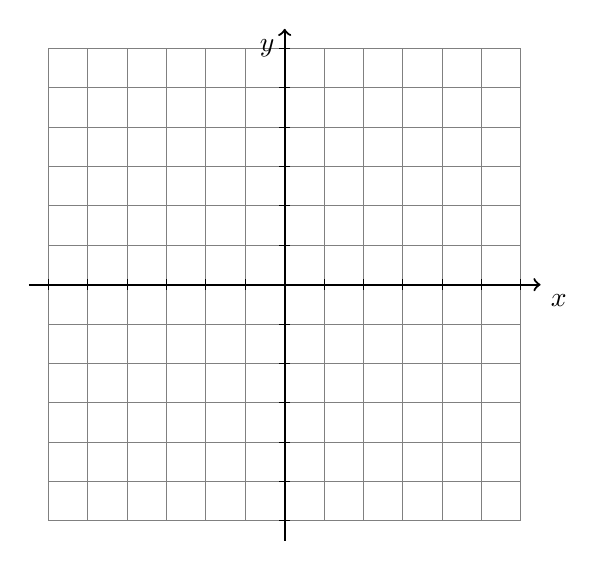
\begin{tikzpicture}[y=.5cm, x=0.5cm,font=\sffamily]
    %% ticks
    \draw[step = 1, gray] (-6,-6) grid (6,6);
    %% axis
    \draw[thick,->] (-6.5,0) -- coordinate (x axis mid) (6.5,0) node[anchor = north west] {$x$};
    \draw[thick,->] (0,-6.5) -- coordinate (y axis mid) (0,6.5) node[anchor = north east] {$y$};
    \foreach \y in {-6,-5,...,-1,1,2,...,6} {
      \draw (2pt, \y) -- (-2pt, \y);
    }
    \foreach \x in {-6,-5,...,-1,1,2,...,6} {
      \draw (\x,2pt) -- (\x,-2pt);
    }

  \end{tikzpicture}

\item Determine the domain and range of $f(x)$.\\[.5in]
\end{enumerate}


\newpage
\item Determine whether the lines $y= 2x+3$ and and $x-3y-5=0$ are parallel, perpendicular, or neither. \vfill


\item Determine an equation of the \emph{vertical} line which passes through the point $(-2, 3)$. Then determine an equation of the \emph{horizontal} line through $(-2,3)$.\vfill

\newpage

\item Consider the function $f(x)=x^2-3x+2$.
\begin{enumerate}
\item Algebraically determine the average rate of change of $f(x)=x^2-3x+2$ between $x_1=1$ and $x_2=3$.
\vfill



\item The graph of $f(x)=x^2-3x+2$ is given below.  Draw a line between the points $(1,f(1))$ and $(3,f(3))$.\\

%\begin{tikzpicture}[scale=1]
%	\begin{axis}[
%	                   axis equal,
%	                   axis line style = thick,
%	                   axis x line=middle, 
%	                   axis y line=center, 
%	                   minor tick num = 3,
%	                   grid = both,
%	                   major grid style={black!70},
%	                   minor grid style ={gray!70},
%	                   xtick={-4,-2,0,2,4,6},
%	                   ytick={-2,0,2,4,6,8},
%	                   xmin = -4,
%	                   xmax = 6,
%	                   ymin = -2.25,
%	                   ymax = 8.25,
%	                   tick align=outside,
%	                   style={font=\tiny}]
%
%		\addplot+[mark=none,smooth, style={thick}] (\x,{\x*\x-3*\x+2});
%		\addplot[only marks, style={mark size=1pt}] table {
%		0 2
%		1 0
%		1.5 -.25 
%		2 0
%		};
%	\end{axis}
%\end{tikzpicture}

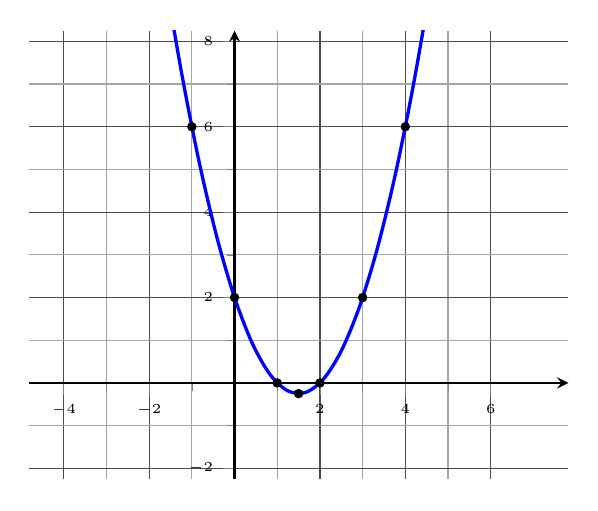
\begin{tikzpicture}[scale=1]
	\begin{axis}[
	                   axis equal,
	                   axis line style = thick,
	                   axis x line=middle, 
	                   axis y line=center, 
	                   minor tick num = 1,
	                   grid = both,
	                   major grid style={black!70},
	                   minor grid style ={gray!70},
	                   xtick={-4,-2,0,2,4,6},
	                   ytick={-2,0,2,4,6,8},
	                   xmin = -3,
	                   xmax = 6,
	                   ymin = -2.25,
	                   ymax = 8.25,
	                   tick align=outside,
	                   style={font=\tiny}]

		\addplot+[mark=none,smooth, style={very thick}] (\x,{\x*\x-3*\x+2});
		\addplot[only marks, style={mark size=1.5pt}] table {
		0 2
		1 0
		1.5 -.25 
		2 0
		3 2
		4 6
		-1 6
		};
	\end{axis}
\end{tikzpicture}

\item Find the slope of the line between the points $(1,f(1))$ and $(3,f(3))$ on $f(x)=x^2-3x+2$.
\vfill
\item What do you notice about the slope of the line between the
  points $(1,f(1))$ and $(3,f(3))$ on $f(x)=x^2-3x+2$ and the average
  rate of change of $f(x)=x^2-3x+2$ between $x_1=1$ and $x_2=3$.
  Why is this?
\end{enumerate}

\clearpage

\item The equations for two different lines are the
  following:
  \begin{eqnarray*}
    \mathrm{Line~1:~} y-3 & = & 4 (x-2), \\
    \mathrm{Line~2:~} y-2 & = & m (x-1),
  \end{eqnarray*}
  where $m$ is a real-valued number.

  \begin{enumerate}
  \item What are the possible values of $m$ that will ensure that the
    two lines intersect? (Provide a justification for your answer.)

    \vfill
  
  \item If you are given that the values of $y$ for the points on the
    graph of line 2 are greater than those of line 1 when $x$ is positive
    what does that imply about the possible values that $m$ could be?
    (Provide a justification for your answer.)
    \sideNote{Make a rough sketch of the graphs representing this situation.}

    \vfill

  \item What values of $m$ will ensure that the $y$ values on the
    graph of line 1 will be less that those on the graph of line 2
    when $x>3$?

    \vfill

  \end{enumerate}

\clearpage
\item The equation for a linear function is given by:
  \begin{eqnarray*}
    D(x) & = & m(x-2)+4,
  \end{eqnarray*}
  where $m$ is a constant. Answer each question below and provide
  a brief justification for your answer.

  \begin{enumerate}
  \item For what values of $m$ is $D(x)$ an increasing function?
    \vfill
  \item For what values of $m$ is $D(x)$ a decreasing function?
    \vfill
  \item What values of $m$ will ensure that $D(3)>5$?
    \vfill
  \item If you are given that the value of $D(x)$ increases by 3 as
    $x$ increases by 6, what is the value of $m$? 
    \vfill
  \end{enumerate}


\end{enumerate}



\hwTitle{Section 1.4}

\begin{enumerate}
\item Consider the line $x+2y=3$.
  \begin{enumerate}
  \item Find the $x$ and $y$ intercepts of the line.
  \item Determine the distance between the $x$-intercept and the $y$-intercept.
  \item Find the slope of the line $x+2y=3$.
  \end{enumerate}

\item The questions below refer to the linear functions shown in the
  plot below. The function $f(x)=m_f x + b_f$ is shown with a solid
  line, the function $g(x)=m_g x + b_g$ is shown with a dashed line,
  and the function $h(x) = m_h x + b_h$ is shown with a dotted line.

  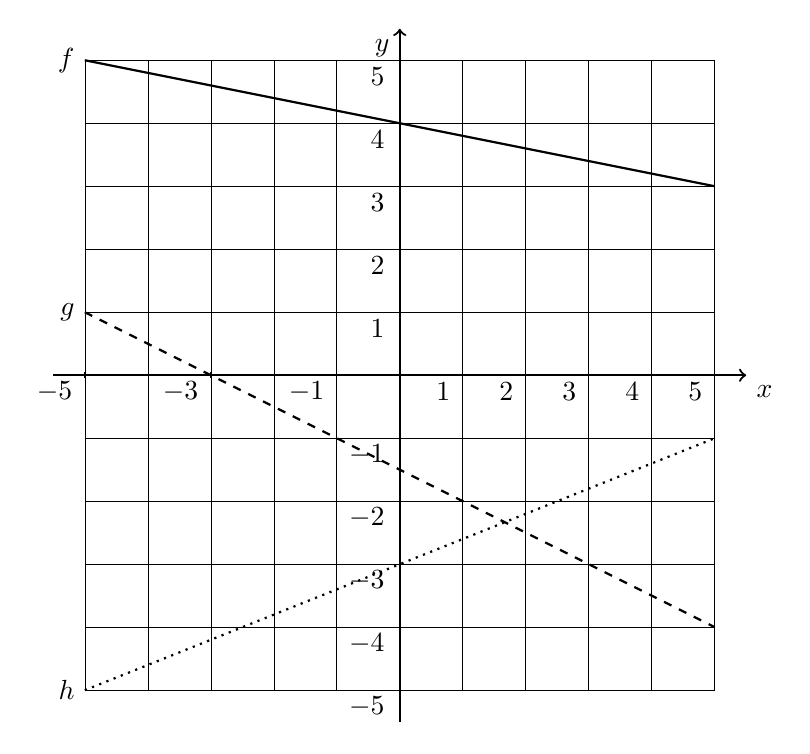
\begin{tikzpicture}[y=0.8cm, x=0.8cm,font=\sffamily]
    %% ticks
    \draw[step = 1, very thin] (-5, -5) grid ( 5,5);
    % axis
    \draw[thick,->] (-5.5,0) -- coordinate (x axis mid) (5.5,0) node[anchor = north west] {$x$};
    \draw[thick,->] (0,-5.5) -- coordinate (y axis mid) (0,5.5) node[anchor = north east] {$y$};
    \foreach \y in {-5,-4,...,-1,1,2,...,5} {
      \draw (1pt, \y) -- (-1pt, \y) node[yshift=-6,xshift=-1,anchor=east] {$\y$};
    }
    \foreach \x in {-5,-3,...,-1,1,2,...,5} {
      \draw (\x,1pt) -- (\x,-1pt) node[yshift=-5,xshift=-1,anchor=east] {$\x$};
    }

    \begin{scope}
      %\clip(-4,-1) rectangle (8,5);
      \draw[thick,solid]  (-5, 5) node[anchor = east] {$f$}  -- (5, 3);
      \draw[thick,dashed] (-5, 1) node[anchor = east] {$g$}  -- (5,-4);
      \draw[thick,dotted] (-5,-5) node[anchor = east] {$h$}  -- (5,-1);
    \end{scope}

  \end{tikzpicture}

  \begin{enumerate}
    \item Determine which $y$-intercept ($b_f$, $b_g$, and $b_h$)
    is the largest and which is the lowest. (Recall that a negative
    number is less than a positive number.) Provide a brief
    justification for your conclusion based on the graph.

    \item Determine which slopes ($m_f$, $m_g$, and $m_h$) is the
    largest and which is the lowest.  Provide a brief justification
    for your conclusion based on the graph.

    \item Determine which function has the highest $x$-intercept
    and which function has the lowest $x$-intercept. Provide a brief
    justification for your conclusion based on the graph.

  \end{enumerate}

\item The equations for two different linear functions are the
  following:
  \begin{eqnarray*}
    \mathrm{Line~1:~} A(x) & = & 5(x+1)-7, \\
    \mathrm{Line~2:~} B(x) & = & m(x+1)-6,
  \end{eqnarray*}
  where $m$ is a constant. Answer each question below and provide
  a brief justification for your answer.

  \begin{enumerate}
  \item For what values of $m$ does the function $B(x)$ increase?
  \item For what values of $m$ does the function $B(x)$ decrease?
  \item For what values of $m$ do the two lines intersect?
  \item For what values of $m$ is $A(x)>B(x)$ for positive values of
    $x$?
  \item For what values of $m$ is $A(x)<B(x)$ for positive values of
    $x$?
  \end{enumerate}

\end{enumerate}
